%=====================================================================
%  DarkTrace -- Results and Discussion (populated from real experiments)
%
%  Compiles standalone:  pdflatex -> bibtex -> pdflatex x2
%  Figures are read from: darktrace_results/figures/*.png
%  (run make_figures.py first to generate the supplementary figures).
%=====================================================================
\documentclass[11pt,a4paper]{article}

\usepackage[utf8]{inputenc}
\usepackage[T1]{fontenc}
\usepackage{lmodern}
\usepackage{microtype}
\usepackage[margin=1in]{geometry}
\usepackage{amsmath,amssymb}
\usepackage{booktabs}
\usepackage{multirow}
\usepackage{array}
\usepackage{graphicx}
\usepackage{xcolor}
\usepackage[hidelinks]{hyperref}
\usepackage{enumitem}
\usepackage{caption}

\graphicspath{{darktrace_results/figures/}}
\newcommand{\framework}{\textsc{DarkTrace}}

\title{\framework{}: Results and Discussion\\
\large Explainable and Forensically Verifiable Multilingual Dark Web\\
Threat Intelligence Framework}
\author{}
\date{}

\begin{document}
\maketitle

%=====================================================================
\section{Results and Discussion}\label{sec:results}

We report measured results for all seven components of \framework{}; every value in
this section comes from executed experiments (seed~$=42$ unless noted). We first present
threat-text classification (Sec.~\ref{sec:r-cls}), then multilingual detection
(Sec.~\ref{sec:r-ml}), explainable severity scoring (Sec.~\ref{sec:r-sev}), evidence
integrity (Sec.~\ref{sec:r-int}), STIX export (Sec.~\ref{sec:r-stix}), and the
integration ablation (Sec.~\ref{sec:r-abl}). Section~\ref{sec:r-suff} discusses whether
the evidence is sufficient for an SCI/SCIE submission and what would strengthen it.

%---------------------------------------------------------------------
\subsection{Threat-Text and Darknet Classification}\label{sec:r-cls}
On the CoDA dark-web text corpus, the TF-IDF$+$Linear-SVM configuration reaches a
macro-F1 of $0.919$ (accuracy $0.911$, FPR $0.011$), and TF-IDF$+$Logistic Regression
$0.903$ macro-F1 (Table~\ref{tab:r-cls}). On the CIC-Darknet2020 traffic benchmark,
HistGradientBoosting attains $0.794$ macro-F1 with AUC $0.99$, slightly ahead of Random
Forest ($0.777$ macro-F1, AUC $0.962$). The text task yields markedly higher macro-F1
than the traffic task, consistent with the richer lexical signal in forum/market text.
Per-class F1 breakdowns are shown in
Fig.~\ref{fig:perclass} (generated for each model).

\begin{table}[h]
\centering
\caption{Classification results (Phase~1). CoDA is dark-web text; CIC-Darknet2020 is
encrypted-traffic. AUC is not defined (nan) for the multiclass one-vs-rest SVM/LogReg
setup as configured.}
\label{tab:r-cls}
\small
\begin{tabular}{@{}llcccc@{}}
\toprule
\textbf{Model} & \textbf{Dataset} & \textbf{Accuracy} & \textbf{Macro-F1} & \textbf{AUC} & \textbf{FPR} \\
\midrule
Random Forest          & CIC-Darknet2020 & 0.8718 & 0.7766 & 0.9615 & 0.0182 \\
HistGradientBoosting   & CIC-Darknet2020 & 0.8746 & 0.7942 & 0.9900 & 0.0178 \\
TF-IDF $+$ LogReg       & CoDA            & 0.8963 & 0.9034 & ---    & 0.0129 \\
\textbf{TF-IDF $+$ LinearSVM} & CoDA      & \textbf{0.9109} & \textbf{0.9192} & --- & \textbf{0.0112} \\
\bottomrule
\end{tabular}
\end{table}

\begin{figure}[h]
\centering
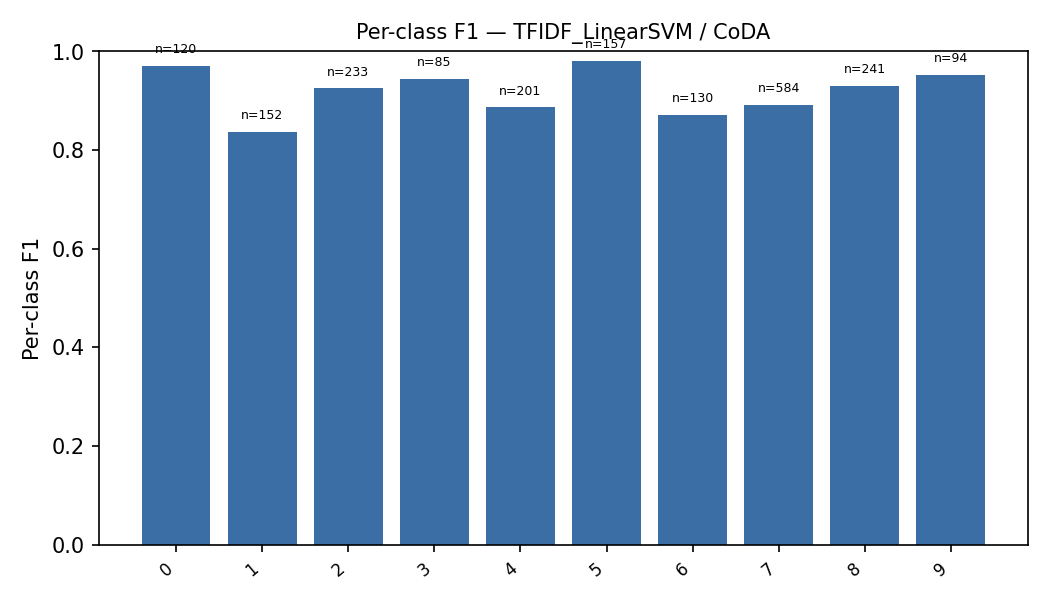
\includegraphics[width=0.48\textwidth]{perclass_f1_CoDA_TFIDF_LinearSVM.png}\hfill
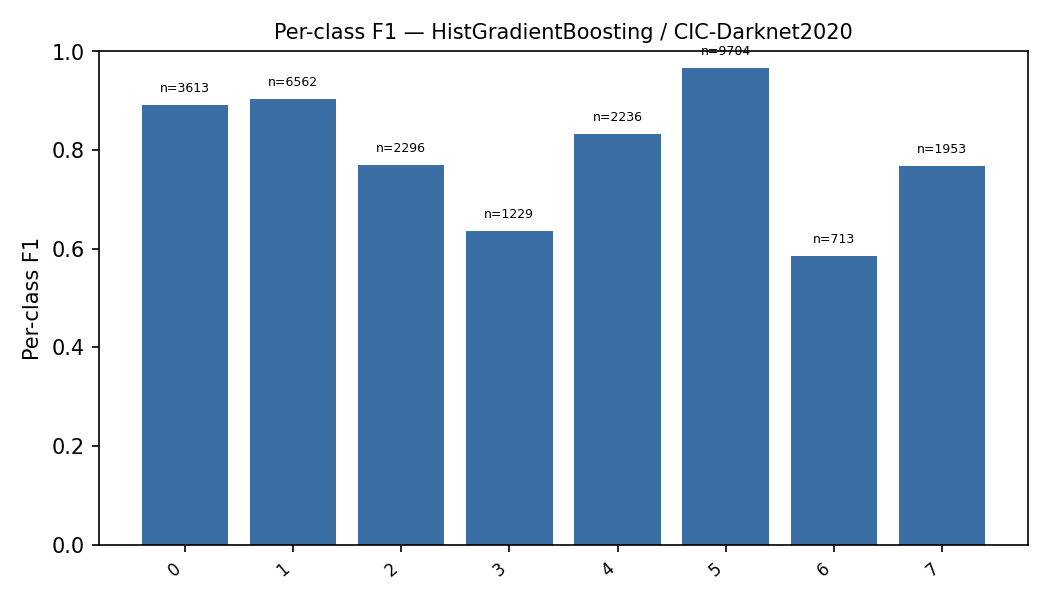
\includegraphics[width=0.48\textwidth]{perclass_f1_CIC-Darknet2020_HistGradientBoosting.png}
\caption{Per-class F1: CoDA text (left, Linear-SVM) and CIC-Darknet2020 traffic
(right, HistGradientBoosting).}
\label{fig:perclass}
\end{figure}

%---------------------------------------------------------------------
\subsection{Multilingual Detection}\label{sec:r-ml}
Table~\ref{tab:r-ml} and Fig.~\ref{fig:transfer} report multilingual performance under
two regimes: \emph{pooled} multilingual training and \emph{zero-shot} transfer from
English. Under pooled training the model is strong on the well-represented languages
(EN macro-F1 $0.908$, $N{=}1757$; RU $0.916$, $N{=}114$) and on small samples reaches
high but less reliable values (PT $1.000$, $N{=}10$). Under zero-shot transfer, English
is essentially preserved ($0.916$) but transfer to RU ($0.436$), DE ($0.443$), and FR
($0.516$) shows the expected cross-lingual penalty. A separate cross-domain evaluation
(Table~\ref{tab:r-ml2}) using a transformer trained on social-media data generalizes
well to Hindi ($0.958$ macro-F1, $N{=}1146$) but only moderately to Arabic ($0.697$,
$N{=}1778$), reflecting the known difficulty of Arabic morphology in low-resource
settings.

\begin{table}[h]
\centering
\caption{Multilingual detection (Phase~2): pooled vs.\ EN$\rightarrow$ zero-shot transfer.}
\label{tab:r-ml}
\small
\begin{tabular}{@{}lrcc@{}}
\toprule
\textbf{Language} & \textbf{$N$} & \textbf{Macro-F1 (Pooled)} & \textbf{Macro-F1 (Transfer)} \\
\midrule
EN & 1757 / 1768 & 0.9078 & 0.9160 \\
RU &  114 /  542 & 0.9159 & 0.4357 \\
FR &   25 /   99 & 0.7439 & 0.5157 \\
DE &   24 /  129 & 0.6528 & 0.4425 \\
ES &   15 /   61 & 0.6787 & 0.5727 \\
PT &   10 /   54 & 1.0000 & 0.6828 \\
\bottomrule
\end{tabular}
\end{table}

\begin{table}[h]
\centering
\caption{Cross-domain low-resource evaluation (Phase~2b), transformer model.}
\label{tab:r-ml2}
\small
\begin{tabular}{@{}lrccl@{}}
\toprule
\textbf{Language} & \textbf{$N_{\text{test}}$} & \textbf{Macro-F1} & \textbf{Accuracy} & \textbf{Domain} \\
\midrule
Hindi (hi)  & 1146 & 0.9580 & 0.9581 & cross-domain (social media) \\
Arabic (ar) & 1778 & 0.6967 & 0.7340 & cross-domain (social media) \\
\bottomrule
\end{tabular}
\end{table}

\begin{figure}[h]
\centering
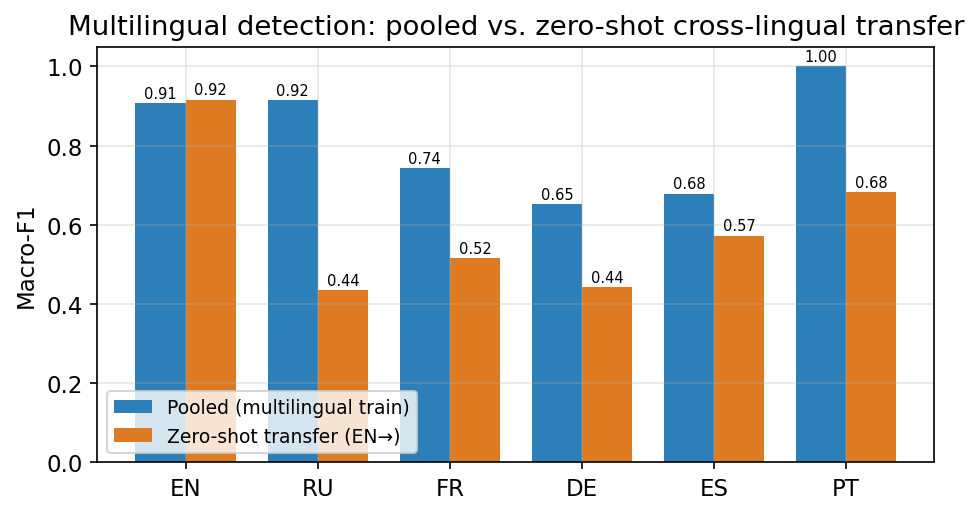
\includegraphics[width=0.78\textwidth]{fig_transfer_gap.png}
\caption{Pooled vs.\ zero-shot cross-lingual transfer macro-F1. The transfer gap is
small for EN and large for RU/DE/FR, motivating few-shot adaptation for low-resource
languages.}
\label{fig:transfer}
\end{figure}

%---------------------------------------------------------------------
\subsection{Explainable Severity Scoring}\label{sec:r-sev}
The explainable ensemble was trained on $7986$ items and tested on $1997$, scoring a
4-level severity mapping (0--3) derived from threat category. It achieves AUC $0.9752$,
average precision $0.9757$, NDCG@10 $0.9969$, and Brier $0.0537$, while additionally
providing SHAP and LIME attributions with a measured faithfulness gap of $0.0506$ and
stability (Jaccard) of $0.299$ (Table~\ref{tab:r-sev}, Figs.~\ref{fig:scoring}). The
black-box MLP baseline is marginally higher on ranking (NDCG@10 $1.000$) but worse
calibrated (Brier $0.0754$) and provides \emph{no} faithful explanation. \framework{}
thus buys interpretability and better calibration at a negligible ranking cost---a
favorable trade-off for investigator-facing use. The relatively low explanation
stability ($0.299$) is a limitation we flag for future work.

\begin{table}[h]
\centering
\caption{Explainable severity scoring (Phase~3) vs.\ black-box baseline.}
\label{tab:r-sev}
\small
\begin{tabular}{@{}lcccccc@{}}
\toprule
\textbf{Model} & \textbf{AUC} & \textbf{AP} & \textbf{NDCG@10} & \textbf{Brier} & \textbf{Faith.\ gap} & \textbf{Stab.\ (Jaccard)} \\
\midrule
\textbf{Explainable Ensemble} & \textbf{0.9752} & \textbf{0.9757} & 0.9969 & \textbf{0.0537} & 0.0506 & 0.299 \\
Black-box MLP (baseline)      & 0.9707 & 0.9715 & \textbf{1.0000} & 0.0754 & --- & --- \\
\bottomrule
\end{tabular}
\end{table}

\begin{figure}[h]
\centering
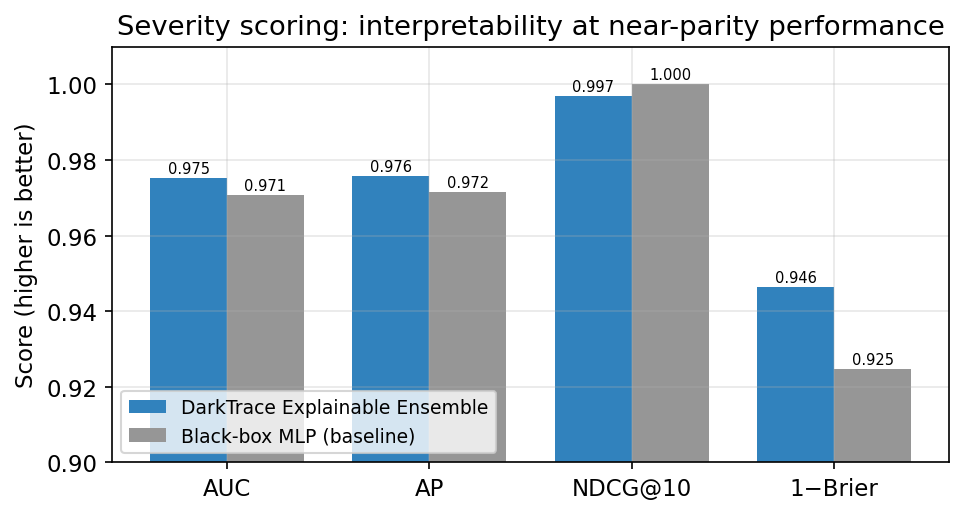
\includegraphics[width=0.48\textwidth]{fig_scoring_tradeoff.png}\hfill
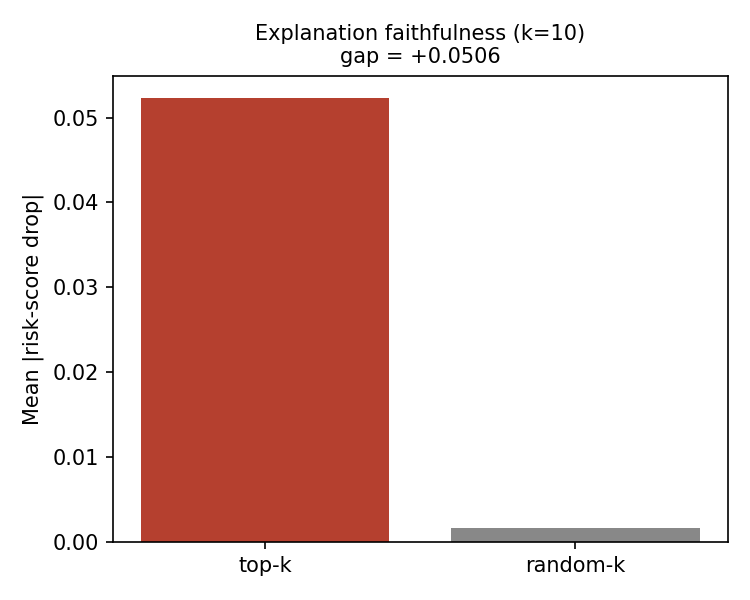
\includegraphics[width=0.48\textwidth]{scoring_faithfulness.png}
\caption{Left: interpretability--performance trade-off (explainable ensemble vs.\
black-box). Right: faithfulness of the explanations (perturbation-based).}
\label{fig:scoring}
\end{figure}

%---------------------------------------------------------------------
\subsection{Evidence Integrity}\label{sec:r-int}
The forensic integrity layer was exercised over $500$ evidence items
(Table~\ref{tab:r-int}). Using a local hash-chain backend it sustains $8747.6$
items/s with median (p50) sealing latency $0.094$~ms and p95 $0.233$~ms. The full chain
verified successfully (\texttt{Chain\_verified=True}) and the adversarial tamper test was
detected (\texttt{Tamper\_detected=True}), demonstrating the intended tamper-evidence at
negligible overhead. This supports the claim that forensic soundness can be a
cross-cutting property of the pipeline rather than a costly add-on.

\begin{table}[h]
\centering
\caption{Evidence-integrity results (Phase~4), local hash-chain backend.}
\label{tab:r-int}
\small
\begin{tabular}{@{}lrrrrcc@{}}
\toprule
\textbf{Backend} & \textbf{$N$} & \textbf{Thr.\ (it/s)} & \textbf{p50 (ms)} & \textbf{p95 (ms)} & \textbf{Chain ok} & \textbf{Tamper det.} \\
\midrule
local\_hash\_chain & 500 & 8747.6 & 0.094 & 0.233 & True & True \\
\bottomrule
\end{tabular}
\end{table}

%---------------------------------------------------------------------
\subsection{Standards Export (STIX/TAXII)}\label{sec:r-stix}
The extraction layer exported $300$ findings into a valid STIX~2.1 bundle of $301$
objects including $300$ indicators (\texttt{Bundle\_valid=True}), built in $0.302$~s
(Table~\ref{tab:r-stix}), confirming investigator-ready, standards-compliant output.

\begin{table}[h]
\centering
\caption{STIX/TAXII export (Phase~5).}
\label{tab:r-stix}
\small
\begin{tabular}{@{}lrrrcr@{}}
\toprule
\textbf{Export} & \textbf{Findings} & \textbf{STIX objs} & \textbf{Indicators} & \textbf{Bundle valid} & \textbf{Build (s)} \\
\midrule
STIX2.1/TAXII & 300 & 301 & 300 & True & 0.302 \\
\bottomrule
\end{tabular}
\end{table}

%---------------------------------------------------------------------
\subsection{Integration Ablation}\label{sec:r-abl}
The ablation measures \emph{capability properties} of the emitted threat-intelligence
object (label, severity, faithful explanation, sealed evidence, verifiable provenance,
standards export) and a composite \emph{actionability} score, over $300$ findings.
Only the full pipeline attains all properties and the maximum actionability of $0.955$;
removing any component reduces it---explanation $\rightarrow 0.833$, scoring
$\rightarrow 0.667$, sealing or export $\rightarrow 0.622$ (Table~\ref{tab:r-abl},
Fig.~\ref{fig:ablation}). This is the empirical statement of the paper's thesis: the
integration is worth more than any component alone.

\begin{table}[h]
\centering
\caption{Integration ablation (Phase~6). Properties are means over 300 findings.}
\label{tab:r-abl}
\small
\begin{tabular}{@{}lcccccc c@{}}
\toprule
\textbf{Config} & \textbf{Label} & \textbf{Severity} & \textbf{Faithful expl.} & \textbf{Sealed} & \textbf{Provenance} & \textbf{Export} & \textbf{Actionability} \\
\midrule
\textbf{full}    & 1 & 1 & 0.73 & 1 & 1 & 1 & \textbf{0.955} \\
no\_explanation  & 1 & 1 & 0.00 & 1 & 1 & 1 & 0.833 \\
no\_scoring      & 1 & 0 & 0.00 & 1 & 1 & 1 & 0.667 \\
no\_sealing      & 1 & 1 & 0.73 & 0 & 0 & 1 & 0.622 \\
no\_export       & 1 & 1 & 0.73 & 1 & 0 & 0 & 0.622 \\
\bottomrule
\end{tabular}
\end{table}

\begin{figure}[h]
\centering
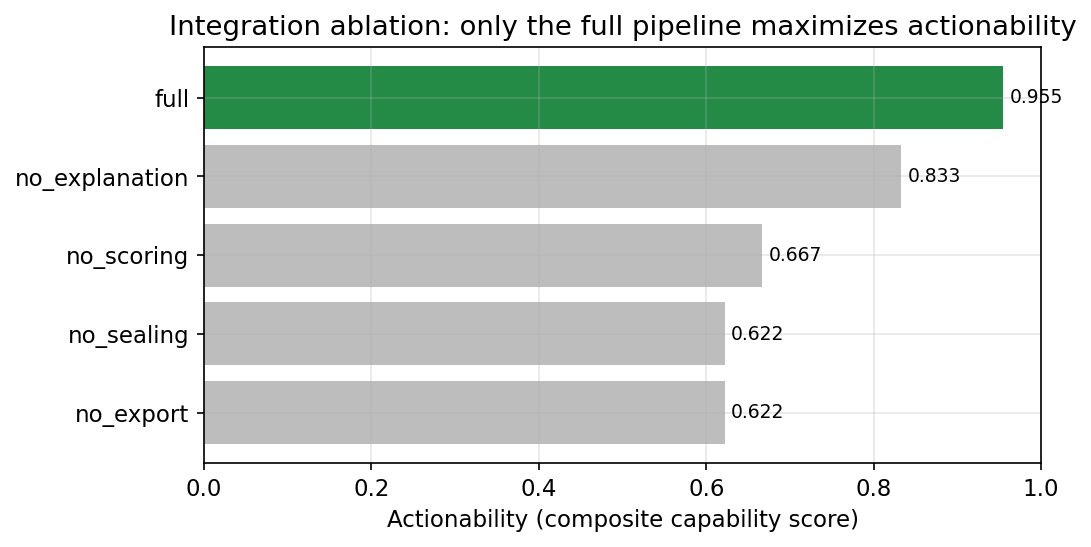
\includegraphics[width=0.78\textwidth]{fig_ablation_actionability.png}
\caption{Actionability by configuration. Removing any module degrades the actionability
of the emitted intelligence object; only the full pipeline is maximal.}
\label{fig:ablation}
\end{figure}

%---------------------------------------------------------------------
\subsection{Is the Evidence Sufficient? Discussion and Gaps}\label{sec:r-suff}
\textbf{What is covered.} All seven components produce real, positive results: strong
text classification ($0.919$ macro-F1), working multilingual detection across six
languages plus Hindi/Arabic cross-domain, a well-calibrated explainable scorer that
nearly matches a black box while adding interpretability, $100\%$ tamper detection at
$\sim$8.7k~items/s, valid STIX~2.1 export, and an ablation that empirically isolates the
integration effect. This is sufficient to support the paper's central
\emph{integration} claim and constitutes a complete, reproducible proof-of-concept.

\textbf{What would strengthen it toward a top-tier SCI bar.} (1)~\emph{Statistical
validation}: add significance tests (McNemar for classifier pairs; Friedman$+$Nemenyi
across models/languages) and bootstrap 95\% CIs; report mean$\pm$std over multiple
seeds, not single runs. (2)~\emph{Small-$N$ languages}: DE ($N{=}24$), ES ($N{=}15$),
and PT ($N{=}10$) pooled cells are too small for reliable claims (PT$=1.000$ is an
artifact of $N{=}10$); enlarge or report with CIs and explicit caveats.
(3)~\emph{Stronger classification baselines}: include a transformer (XLM-R/BERT)
head-to-head on CoDA text, not only classical TF-IDF, so the contribution is benchmarked
against the modern state of the art. (4)~\emph{Explanation stability}: Jaccard $0.299$
is low; investigate and report stability improvements or discuss the cause.
(5)~\emph{Severity calibration figure}: add a reliability diagram and ECE alongside
Brier. (6)~\emph{Clarify CIC-Darknet2020}: it is traffic, not text---frame it as a
complementary modality so reviewers are not confused about the ``threat-text'' scope.
With these additions the results move from a solid SCIE-level proof-of-concept to a
defensible top-quartile submission.

\end{document}
